\chapter{Theory}

    The Standard Model (SM) of particle physics has proven excellent at describing particle interactions up to the energy scale of modern colliders ($\sim$~TeV) and with the discovery of a Standard Model like Higgs Boson at the Large Hadron Collider (LHC) the theory will be able to claim completeness up to the energy scale of modern colliders. However the Standard Model is known to be incomplete, with observations such as neutrino mass, the lack of anti-matter in the observable universe and the lack of a quantum gravity description with the related hierarchy problem\footnote{The hierarchy problem highlights the drastic difference in force strength between gravity and the other fundamental forces seen in the standard model}, the Standard Model is far from a theory of Everything. This then leaves the possibility of new physics beyond the SM that could appear in the energy scope of the LHC.
    % maybe history of finding composite particles.

\section{Standard Model}
    
    The Standard Model of particle physics is is a quantum field theory describing the interaction of particles and forces at a fundamental level. These forces and particles are so far seen to be the most fundamental components in nature describing all knows quantum systems but with the absence of gravity. Particles are split between fermions the particles composing matter and bosons the force carriers in the model. The bosons are split between the three fundamental forces Strong, Weak and Electromagnetic while the fermions are split in to two different categories leptons and quarks according to which forces they interact with. Fermions have the property of having spin 1/2 while bosons however have an integer spin of either 0 or 1. Each particle has an associated anti-particle with opposite charge. 

    \subsubsection*{Leptons}
    Leptons only interact with other particles via the electromagnetic and weak forces. There are 6 leptons in total organised in to 3 flavours, the electron (e), muon ($\mu$) and tau ($\tau$) as well as the neutrinos, electron neutrino ($\nu_{e}$), muon neutrino ($\nu_{\mu}$) and tau neutrino ($\nu_{\tau}$). All the leptons along with their mass and charge can be seen in table \ref{tab:leptons}. It is important to note that the standard model predicts neutrinos to be massless while experiment has proven neutrinos to have mass via observations of neutrino oscillations between flavours. 


    \begin {table}[h]
        \begin{center}
        \begin{tabular}{|c|c|c|c|}
            \hline
            \multirow{2}{*}{Charge ($q$)}      & \multicolumn{3}{c|}{Generation} \\
            \cline{2-4}
                                & I     & II    & III   \\
            \hline
            \multirow{3}{*}{\Large -1} & electron & muon & tau \\
                                & {\Huge e}     & {\Huge $\mu$} & {\Huge $\tau$} \\
                                & m = 0.51 MeV  & m = 105.7 MeV & m = 1.777 GeV \\
            \hline
            \multirow{3}{*}{\Large 0} & electron neutrino & muon neutrino & tau neutrino \\
                                & {\Huge $\nu_{e}$} & {\Huge $\nu_{\mu}$} & {\Huge $\nu_{\tau}$}     \\
                                & m $<$ 2.2 eV      & m $<$ 0.17 MeV      & m $<$ 15.5 MeV \\
            \hline
        \end{tabular}
        \caption{Table showing the leptons found in the Standard Model.}
        \label{tab:leptons}
        \end{center}
    \end {table}
 
    \subsubsection*{Quarks}
    Quarks interact with other particles via all three forces electromagnetic, weak and strong. Again there are 6 quarks organised in to 3 flavours, up (u), down (d), charm (c), strange (s), top (t) and bottom (b). All the quarks along with properties mass and charge can be seen in table \ref{tab:quarks}. Quarks also come with a property called colour charge important in how the strong interaction works. The strong force leads to the property called colour confinement found in quarks causing quarks to hadronise quickly with only colour neutral particles seen. These colour neutral or ``colourless'' particles referred to as hadrons are composed of quarks and come in two configurations baryons and mesons with three and two quarks each respectively. Protons and neutrons are baryons containing the quark configurations uud and udd which appear within the nucleus of atoms. Many other configurations of quarks form different baryons but none are stable. Mesons are composed of one quark and one anti-quark but none are found to be stable in nature. 

    \begin {table}[h]
        \begin{center}
        \begin{tabular}{|c|c|c|c|}
            \hline
            \multirow{2}{*}{Charge ($q$)}      & \multicolumn{3}{c|}{Generation} \\
            \cline{2-4}
                                & I     & II    & III   \\
            \hline
            \multirow{3}{*}{\Large $+\frac{2}{3}$} & up quark & charm quark & top quark \\
                                & {\Huge u}             & {\Huge c}             & {\Huge t} \\
                                & m $\approx$ 2.3 MeV   & m $\approx$ 1.275 GeV & m $\approx$ 173.07 GeV \\
            \hline
            \multirow{3}{*}{\Large $-\frac{1}{3}$}  & down quark & strange quark & bottom quark \\
                                & {\Huge d}             & {\Huge s}             & {\Huge b}     \\
                                & m $\approx$ 4.8 eV    & m $\approx$ 95 MeV    & m $\approx$ 4.18 GeV \\
            \hline
        \end{tabular}
        \caption{Table of quarks found in the Standard Model.}
        \label{tab:quarks}
        \end{center}
    \end {table}



    \subsubsection*{Gauge Bosons}
    There are 4 bosons in the standard model as well as the newly observed candidate for the fifth the Higgs Boson. The higgs boson is discussed later but for now will will look at the force carriers or gauge boson's. The gauge boson's consist of the gluon ($g$) carrier of the strong force, the photon ($\gamma$) carrier of the electromagnetic force and then the W and Z bosons carriers of the weak force. All gauge bosons have a spin of 1 with only the W boson having a electric charge and therefore the only particle with a distinguishable particle and antiparticle. All bosons and properties can be seen in table \ref{tab:bosons}.\\

    \begin {table}[h]
      \begin{center}
      \begin{tabular}{|l|c|c|}
         \hline
         Force & Charge & Boson \\
         \hline
         \multirow{3}{*}{Electromagnetic} & \multirow{3}{*}{\Large 0} & photon \\
         & & {\Huge $\gamma$} \\
         & & m = 0 \\
         \hline
         \multirow{6}{*}{Weak} & \multirow{3}{*}{\Large 0} & Z boson \\
         & & {\Huge Z} \\
         & & m = 91.2 GeV \\
         \cline{2-3}
         & \multirow{3}{*}{\Large $\pm1$} & W boson \\
         & & {\Huge W} \\
         & & m = 80.4 GeV \\
         \hline
         \multirow{3}{*}{Strong} & \multirow{3}{*}{\Large 0} & gluon \\
         & & {\Huge g} \\
         & & m = 0 \\
         \hline
      \end{tabular}
      \caption{Table showing the gauge bosons found in the Standard Sodel.}
      \label{tab:bosons}
      \end{center}
    \end {table}



    \subsection{Fundamental Forces}
    The Standard Model is described as a local gauge theory meaning observables remain unchanged under transformations be they global transformations, a uniform transformation over all space and time, or local transformations, a transformation as a function of space and time. This is also described as gauge symmetry or gauge invariance and held as an important trait for quantum field theories to posses. The first fundamental force to gain a gauge theory was Quantum Electrodynamics with the U(1) symmetry referring to a theory symmetric under unitary $1\times1$ group transformations. The weak theory and Quantum Cromodynamics followed with symmetries SU(2) and SU(3) transformations respectively. SU(n) refers to a group of n$\times$n special unitary matrices (Special refers to the matrices all having a determinant of 1). This is why the SM is referred to as a U(1)$\times$SU(2)$\times$SU(3) group theory after the unification of the forces.


    \subsubsection*{Quantum Electrodynamics}
    Quantum Electrodynamics (QED) describes the interactions of the photon with charged fermions. Photons are massless meaning the electromagnetic force has infinite reach. The theory describes the interaction strength between the photon and both quarks and charged leptons. The quantity conserved in these interactions is particle electric charge. QED is important in calculating the $qq \rightarrow\gamma\rightarrow\ell\ell$ process which is a main background to this analysis in the form of Drell-Yan. The photon has no charge so there are no self interactions between photons. The fundamental QED interaction vertex can be seen figure \ref{fig:QED}.

    \begin{figure}[h]
        \begin{center}
        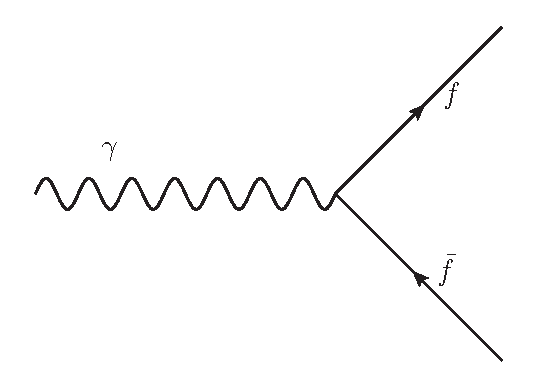
\includegraphics[width=0.5\linewidth]{images/gamma_fermion.eps}
        \end{center}
        \caption{Fundamental QED interaction vertex. Where $f$ can be any charged fermion.}
        \label{fig:QED}
    \end{figure}

    \subsubsection*{The Weak Interaction}
    The Weak interaction describes interactions involving the neutral Z$^{0}$ boson and the charged W$^{\pm}$ boson. These bosons both have mass limiting the range of the weak interaction. 
    %The weak interaction also allows for Charge Parity (CP) violation via the W$^{\pm}$ boson. This process is a quark flavour changing current and the Cabibbo Kobayashi Maskawa (CKM) matrix defines the relative coupling strengths of each flavour changing interaction between the quarks.
    This theory allows for the interaction between all fermions including neutrinos (which only interact via the weak force) and self interaction between Z and W bosons. This is important for this analysis because of the diboson background to signal consisting of production of ZZ WZ and WW events decaying to electrons as well a simple Z boson decaying to two electrons. The fundamental weak interaction vertices can be seen in figure \ref{fig:weak}.

    \begin{figure}[h]
        \begin{center}
        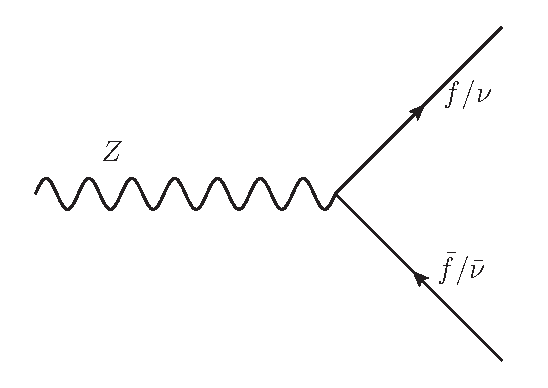
\includegraphics[width=0.329\linewidth]{images/Z_fermion.eps}
        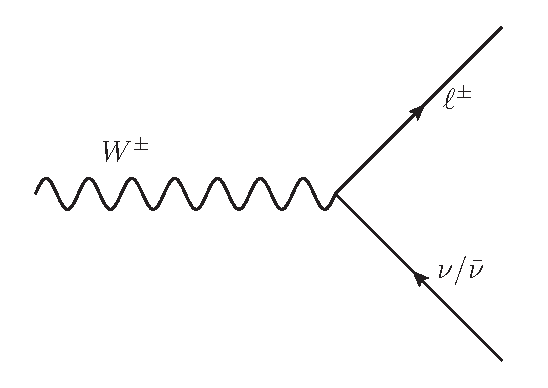
\includegraphics[width=0.329\linewidth]{images/W_lepton.eps}
        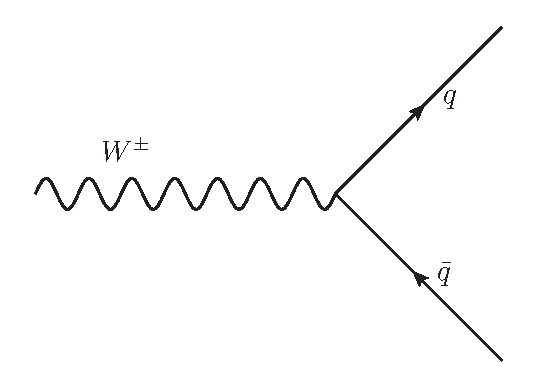
\includegraphics[width=0.329\linewidth]{images/W_quark.eps}\\
        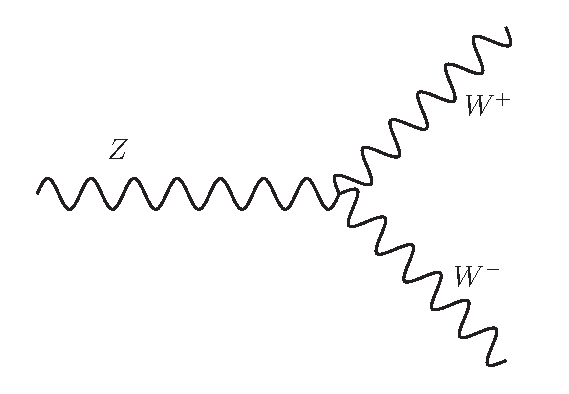
\includegraphics[width=0.33\linewidth]{images/Z_WW.eps}
        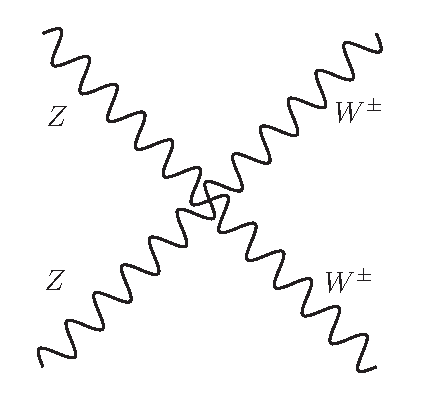
\includegraphics[width=0.25\linewidth]{images/ZZ_WW.eps}
        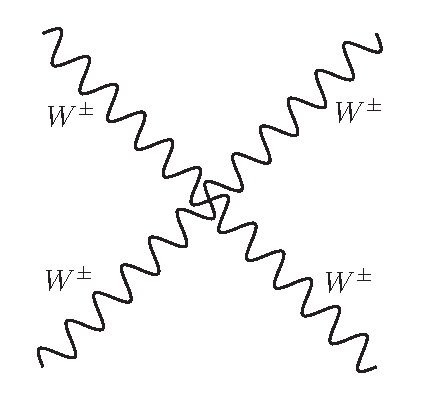
\includegraphics[width=0.25\linewidth]{images/WW_WW.eps}\\
        \end{center}
        \caption{Fundamental weak interaction vertices. Where $f$ can be any charged fermion, $\ell$ can be any charged lepton and $q$ can be any quark as long as charge is conserved in each case.}
        \label{fig:weak}
    \end{figure}

    \subsubsection*{Electroweak Unification \& Symmetry Breaking}
    The electromagnetic and weak theories were united by Glashow, Weinberg and Salam \cite{} showing that at high energy (past the electroweak unification/phase transition energy $\sim246$~GeV) the forces can be considered as one and conserves a combined quantum number, weak hypercharge $Y = I_{3} - Q$ where $I_{3}$ is the weak isospin and $Q$ is the electric charge. This combination of the forces is the U(1)$\times$SU(2) symmetry. This conserved symmetry then gives rise to 4 gauge fields $W^{1}$, $W^{2}$, $W^{3}$ and $B^{0}$. The first three originating from symmetries in SU(2) and the last from U(1). The gauge bosons we observe in experiment are then obtained by a mixing of these gauge fields as found in equations \ref{eq:Wboson} and \ref{eq:Zboson} where $\cos{\theta_{w}}$ = m$_{W}$/m$_{Z}$.
    \begin{equation}
        W^{\pm} = \frac{W^{1} \mp iW^{2}}{\sqrt{2}}
      \label{eq:Wboson}
    \end{equation}
    \begin{equation}
        \left(\begin{array}{c} \gamma \\ Z^{0}\end{array}\right)
          = \left( \begin{array}{cc} 
              \cos\theta_{w} & \sin\theta_{w} \\  
              -\sin\theta_{w} & \cos\theta_{w} \\ 
            \end{array} \right)
            \left(\begin{array}{c} B^{0} \\ W^{3}\end{array}\right)
      \label{eq:Zboson}
    \end{equation}
    However electroweak unification alone causes a problem by predicting W and Z bosons as massless contradicting experimental results and implying electroweak symmetry must be broken. The solution to this problem comes about by the introduction of the Higgs mechanism\cite{}. The Higgs mechanism makes the prediction of a new complex doublet of scalar fields referred to as the Higgs field. This Higgs field has a non zero vacuum expectation value allowing symmetry in the U(1)$\times$SU(2) group at high energy, however below the electroweak phases transition the Higgs potential has a non zero minima we call the vacuum expectations energy. This induces a spontaneous symmetry breaking allowing the weak gauge bosons to have mass while photons remain massless. This Higgs field also gives rise to a massive scalar boson referred to as the Higgs boson. A scalar boson fitting the description of the Higgs boson was recently discovered at the two main LHC experiments proving the existence of electroweak symmetry breaking of this form exists \cite{Aad20121,Chatrchyan201230}. 


    \subsubsection*{Quantum Chromodynamics}
    
    Quantum Chromodynamics (QCD) is the theory associated with the strong force. It describes a interactions between particles conserving a quantum number called colour. The SU(3) symmetric group gives rise to 8 massless gauge bosons referred to as gluons. Gluons interact with only coloured particle which include quarks and themselves. The strong interaction is different in the way it strengthens with increasing distance and weakens to asymptotic freedom at small distances. This increase in interaction strength with increasing distance is referred to colour confinement discussed previously where as quarks separate the interaction energy increases to the point that $q\bar{q}$ pairs form combining again to form colourless baryons and mesons. The fundamental QCD interaction vertices can be seen in figure \ref{fig:QCD}.

    \begin{figure}[h]
        \begin{center}
        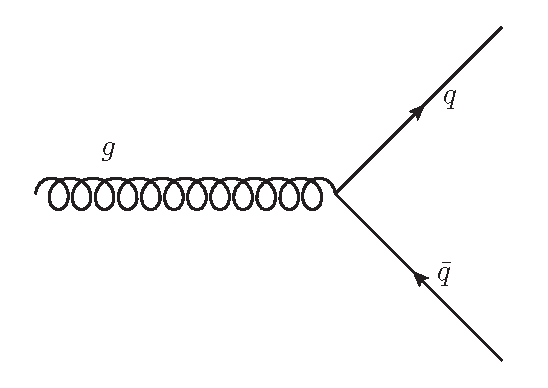
\includegraphics[width=0.34\linewidth]{images/g_quark.eps}
        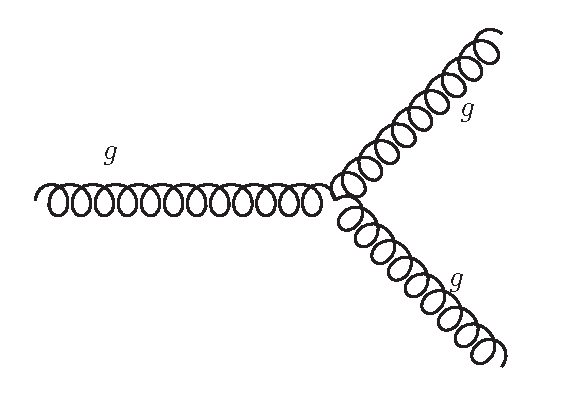
\includegraphics[width=0.34\linewidth]{images/g_gg.eps}
        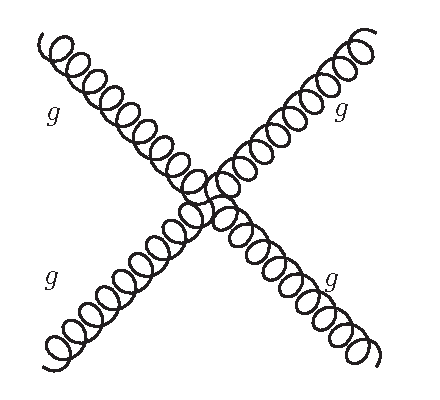
\includegraphics[width=0.25\linewidth]{images/gg_gg.eps}
        \end{center}
        \caption{Fundamental QCD interaction vertices. Where $q$ can be any quark.}
        \label{fig:QCD}
    \end{figure}

    %\subsection{Success and beyond}
    %\subsection{composite particles}



\section{Non-resonant new Physics}

    Beyond the Standard Model (BSM) or new physics models is a staple of the physics programs of the LHC detectors. Any theoretical models not contained within the Standard Model (SM) can fall in to this category and LHC experiments aim to search for as many of these models as are feasible within scope (proton-proton collisions and within the energy range of the LHC). Within the detection channel of two lepton decays (di-lepton) non-resonant signals could be a signature of new physics. This physics would show as a divergence from the SM background prediction in the di-lepton mass spectrum contrasted with resonant signals of particles such as the Z boson which shows as a peak in the di-lepton mass spectrum.

    Non-resonant signals could be the results of many BSM theoretical models but two main theories are presented here and their searches compose the rest of this thesis.


    \subsection{Contact Interaction Theory}
        \label{sec:CItheory}

        The SM assumes quarks and leptons to be fundamental particles in nature. This assumption is not without compelling argument but like the proton beforehand there is no reason quarks and leptons should not be composite structures or bound states of more fundamental particles, often referred to as preons \cite{Eichten:1983hw}, only observable at an energy scale $\Lambda$ we have yet to reach. 

        One way quark and lepton compositeness would exhibit itself is in 4-fermion contact interactions between two quarks from the incoming protons producing two final state leptons ($q\bar{q} \rightarrow \ell^{-}\ell^{+}$). This is the compositeness signal searched for at the ATLAS detector. As can be seen in the Feynman diagrams in figure \ref{fig:fd} 4-fermion contact interaction are indistinguishable from the main background process Drell-Yan.\footnote{Drell-Yan (DY) describes of the annihilation of a quark and antiquark forming a virtual photon or Z boson which then decays in to a lepton pair ($q\bar{q} \rightarrow \gamma^{*}/Z \rightarrow \ell^{-}\ell^{+}$).}

        \begin{figure}[h]
            \begin{center}
            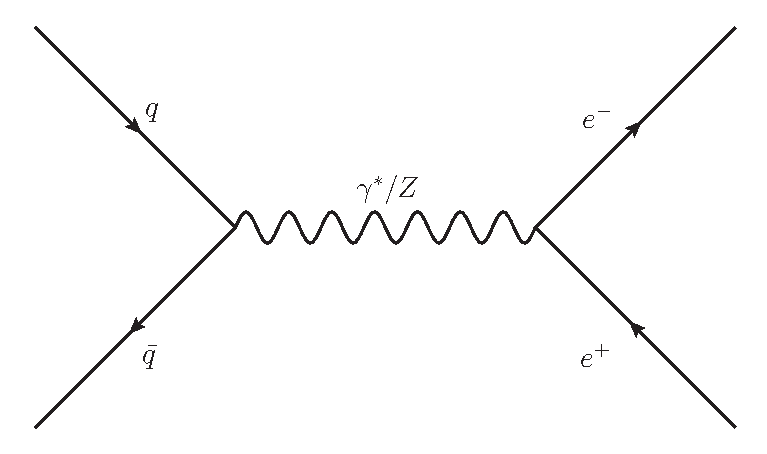
\includegraphics[width=0.45\linewidth]{images/DY_qq_ee.eps}
            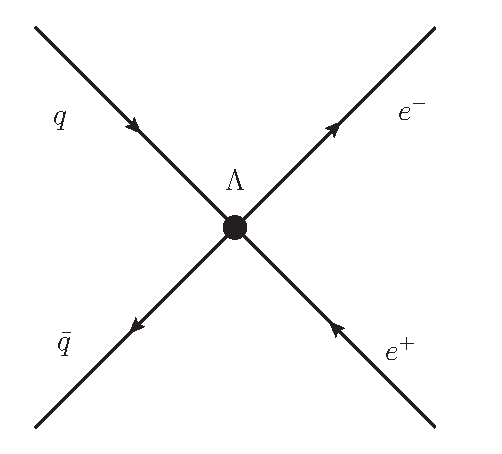
\includegraphics[width=0.3\linewidth]{images/CI_qq_ee.eps}
            \end{center}
            \caption{Feynman diagrams of the predominant background SM process Drell-Yan (left) and by comparison the contact interaction (right).}
            \label{fig:fd}
        \end{figure}

        Without knowing the intermediate process one can write a Lagrangian describing the new interaction:
        \begin{equation}
            \mathcal{L} = \frac{g^{2}}{2\Lambda^{2}}
                [\eta_{LL} (\bar{\psi_{L}}\gamma_{\mu}\psi_{L}) (\bar{\psi_{L}}\gamma^{\mu}\psi_{L}) 
                + \eta_{RR} (\bar{\psi_{R}}\gamma_{\mu}\psi_{R}) (\bar{\psi_{R}}\gamma^{\mu}\psi_{R}) 
                + 2\eta_{LR} (\bar{\psi_{L}}\gamma_{\mu}\psi_{L}) (\bar{\psi_{R}}\gamma^{\mu}\psi_{R}) ]
        \end{equation}
        where $g$ is the coupling constant, $\Lambda$ is the energy scale of new physics and $\psi_{L}$ and $\psi_{R}$ are the left and right handed fermionic fields respectively. The sign of $\eta$ defines whether the new interaction interferes constructively ($\eta = -1$) or destructively ($\eta = +1$) with DY and is always unity. For previous analyses \cite{PhysRevLett.103.191803,PhysRevLett.96.211801,PhysRevD.87.015010} a benchmark model of just the Left-Left (LL) component has been used and is defined by $\eta_{LL} = \pm~1$ and $\eta_{RR} = \eta_{LR} = 0$. This thesis discusses both an analysis searching for only LL and one with an investigation of each of the three parameters. Due to the symmetry of left handed and right handed interactions both the LL and RR cases are predict similar distributions however the LR case exhibits a different angular dependence than either of the other formalisms or the DY background. This difference is the primary reason for the inclusion of the angular search variables described later in the analysis. The discriminating variables used are therefore dilepton invariant mass and cosine of the decay angle $\theta^{*}$. The angle $\theta^{*}$ is defined in the Collins-Soper frame \cite{PhysRevD.16.2219} which is defined with the $x$-axis perpendicular to the incoming parton momentum frame and the $z$-axis bisecting the angle between the two incoming parton momenta. Since the incoming parton information is understandably unavailable the $z$-axis is taken as the direction of the incoming quark (as opposed to anti-quark) obtained from the boost in to the dilepton frame. The angle $\theta^{*}$ is then defined as the angle between this $z$-axis and the momentum of the outgoing negatively charged lepton (or electron in this analysis).

        %diagram of theta *!!!!!!!!!!!!

        Figure \ref{fig:theoryAFB} shows the difference expected between the LR CI models and DY background from a truth Monte-Carlo study. The variables used are forward backwards asymmetry ($A_{FB}$) and dilepton invariant mass, where $A_{FB}$ is defined in relation to cos$\theta^{*}$ as:
        \begin{equation}
            A_{FB} = 
                \frac{N_{F} - N_{B}}{N_{F} + N_{B}}
            \label{eq:AFB}
        \end{equation}
        where $N_{F}$ and $N_{B}$ are number of events found with cos$\theta^{*}$ greater than 0 and less than 0 respectively.
        
        \begin{figure}[h]
            \begin{center}
            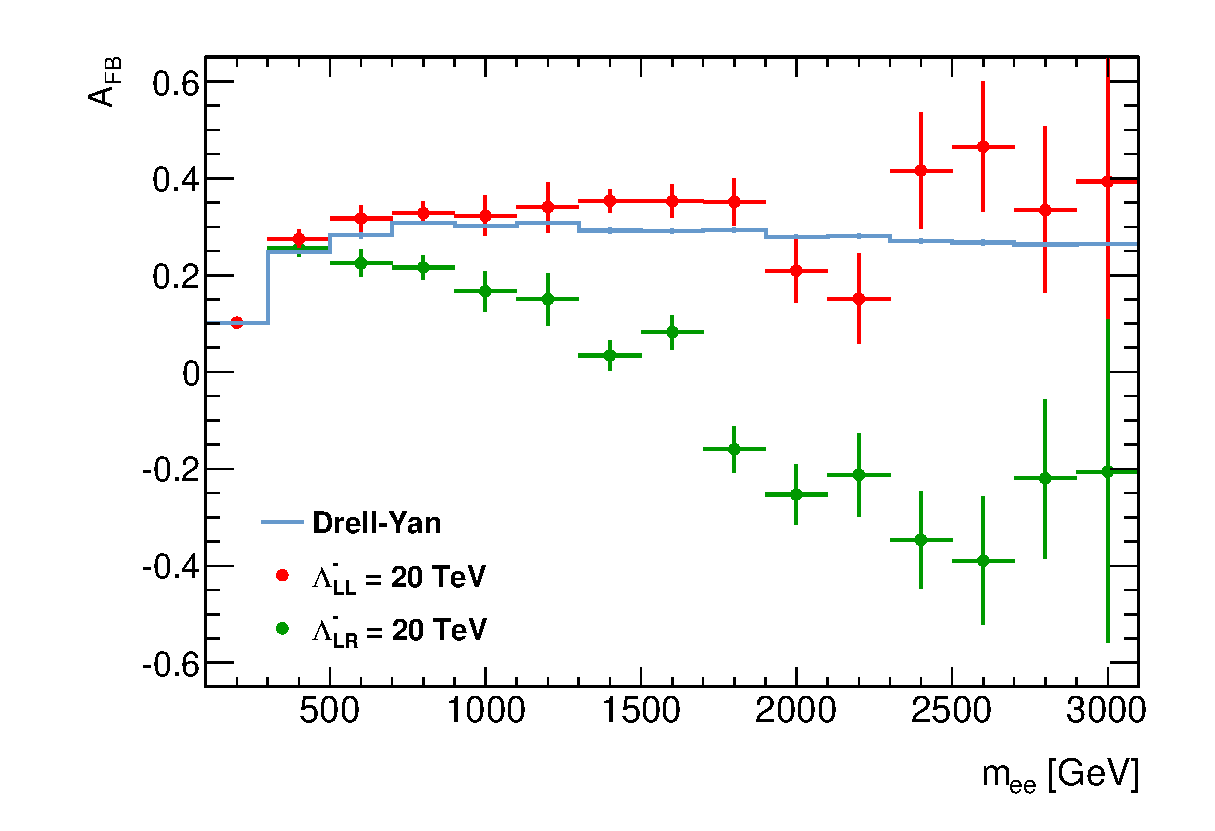
\includegraphics[width=0.9\linewidth]{images/AFB_MC.eps}
            \end{center}
            \caption{Monte-Carlo truth level comparison between the forward backwards asymmetry of DY and and of a CI LR signal.}
            \label{fig:theoryAFB}
        \end{figure}

        A differential cross section for this interaction, $q\bar{q} \rightarrow \ell^{-}\ell^{+}$ ($qq\ell\ell$), is given by
        \begin{equation}
            \frac{d\sigma}{dm_{\ell\ell}} = 
                \frac{d\sigma_{DY}}{dm_{\ell\ell}} 
                - \eta\frac{F_{I}}{\Lambda^{2}} 
                + \frac{F_{C}}{\Lambda^{4}},
            \label{eq:DiffCross}
        \end{equation}
        where $m_{\ell\ell}$ is the dilepton mass and $\Lambda$ is the scale of the new physics. In the case of quark/lepton compositness $\Lambda$ refers to the point at which fermions stop being bound as SM quarks and leptons. $F_{I}$ and $F_{C}$ define the interference DY-CI term and the pure CI term respectively. The scale of the interference and pure term vary with both the dilepton invariant mass as well as the scale of new physics $\Lambda$.

        Experimentally this interaction would be seen as a deviation from the Standard Model Drell-Yan dilepton mass spectrum as seen in figure \ref{fig:theoryInvMass}. 

        \begin{figure}[h]
            \begin{center}
            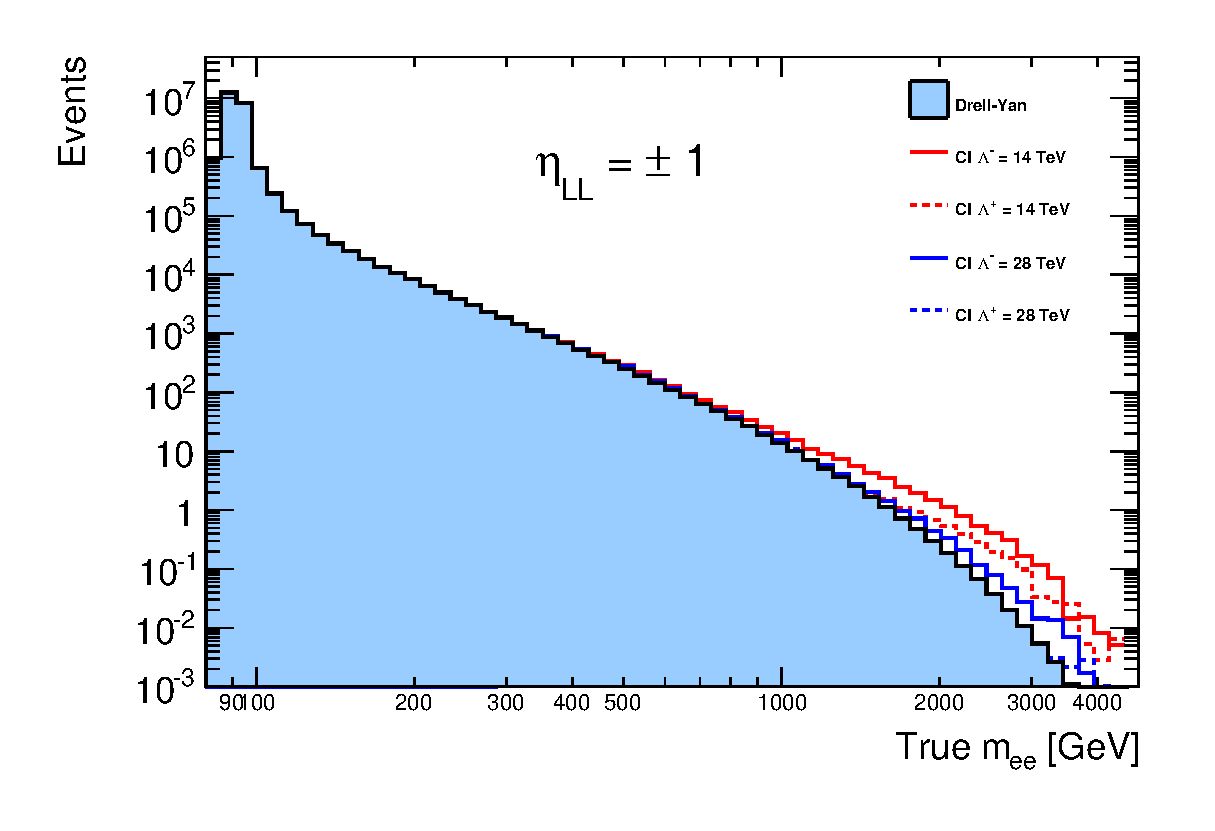
\includegraphics[width=0.9\linewidth]{images/truth_mass_LL.eps}
            \end{center}
            \caption{Monte-Carlo truth level comparison between DY spectrum with and without CI signal.}
            \label{fig:theoryInvMass}
        \end{figure}

    

    \subsection{ADD Theory}
      \label{sec:ADD_T}

        Arkani-Hamed, Dimopoulos, and Dvali (ADD) \cite{ArkaniHamed:1998rs} described a model with large extra dimensions proposed to solve the hierarchy problem and bring the energy scale associated with gravity (the Planck scale M$_{Pl}$ $\sim$ $10^{16}$~TeV) down to the level of electroweak energy scale (M$_{EM}$ $\sim$ $10^{-1}$). This is achieved with the introduction of $n$ additional compactified spacial dimensions with radius $R$. This then gives a new scale in the 4+$n$ dimensional space, M$_{D}$, which is related to the Planck scale by M$_{Pl}$ = M$_{D}^{n+2}R^{n}$. If both the radius of the extra dimensions $R$ and and number $n$ are large enough this solves the hierarchy problem by bringing M$_{D}$ down to the level of M$_{EM}$. Large extra dimensions are distinct from other extra dimensions theories due to their relatively large radius $R$.
        One version of the ADD model proposes a Graviton that propagates the extra dimensions acquiring Kaluza-Klein (KK) modes that show as a broad excess above the SM background. The Graviton is the only propagator in these extra $n$ dimensions with each dimension resulting in a new KK mass splitting of the Graviton mass. The mass splitting occurs with an interval of $1/R$ and since $R$ is required to be large by the theory this pushes the mass splitting together causing a continuous peak like structure analogous to a non-resonant excess. The sum over these virtual KK modes has to be regularised by an ``ultra violet'' cutoff ($\Lambda_{T}$) and it is convention to equate this cutoff to the onset of quantum gravity (M$_{S}$) only below which the theory is valid. The scale M$_{S}$ is used as the scale of new physics for the ADD theory below which ADD is a low energy effective theory. This scale can be related to the new $n$ dimensional Planck scale (M$_{D}$) by:
        \begin{equation}
            M_{S} = 2~\sqrt{\pi}\left[{\Gamma (n/2)}\right]^{1/(n+2)}M_{D}
            \label{eq:gravScale}
        \end{equation}
        where $\Gamma$ is the decay width. Below the scale M$_{S}$ virtual Graviton exchange would lead to a broad excess over the SM Drell-Yan dilepton mass spectrum. A Feynman diagram of this graviton exchange is seen in figure \ref{fig:fdADD}.

        \begin{figure}[h]
            \begin{center}
            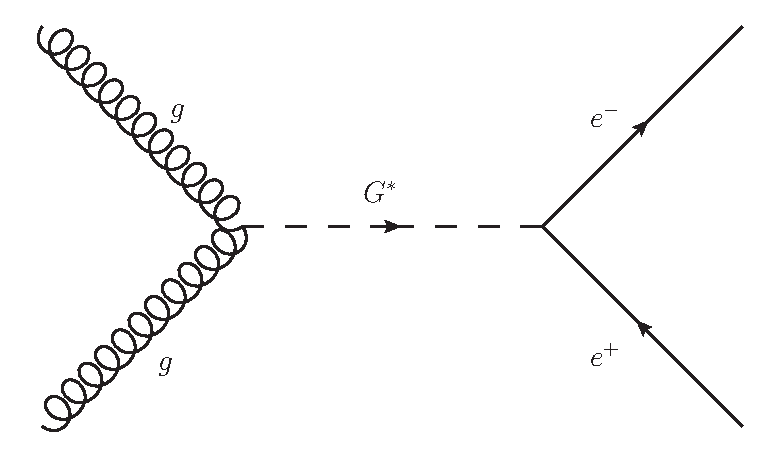
\includegraphics[width=0.45\linewidth]{images/Gvirtual_gg_ee.eps}
            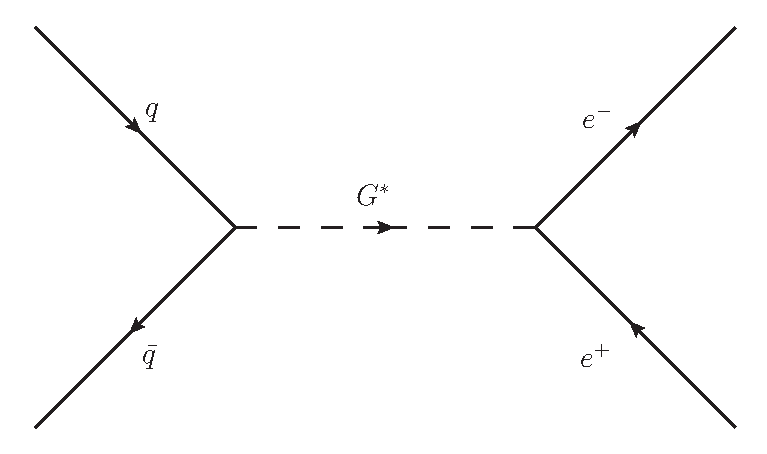
\includegraphics[width=0.45\linewidth]{images/Gvirtual_qq_ee.eps}
            \end{center}
            \caption{Feynman diagram of Graviton exchange in the ADD theory coming from both gluon (left) and quark (right) annihilation.}
            \label{fig:fdADD}
        \end{figure}

        The total differential cross-section for the dilepton SM DY and virtual Graviton exchange is then:
        \begin{equation}
            \frac{d\sigma}{dm_{\ell\ell}} =
                \frac{d\sigma_{DY}}{dm_{\ell\ell}} +
                \mathcal{F}\frac{F_{I}}{M_{S}^{4}} +
                \mathcal{F}^{2}\frac{F_{G}}{M_{S}^{8}}
            \label{eq:ADDcs}
        \end{equation}
        where $\sigma_{DY}$ is the SM DY cross-section, $F_{I}$ and $F_{G}$ are the Graviton-DY interactions term and pure virtual Graviton exchange term respectively while $\mathcal{F}$ is a formalism dependent parameter and also dimensionless. 
        Three formalisms are commonly used to describe ADD theory, these are Giudice, Rattazzi, and Wells (GRW) \cite{Giudice:1998ck}, Han, Lykken, and Zhang (HLZ) \cite{PhysRevD.59.105006} and Hewett \cite{PhysRevLett.82.4765}. Defining $\mathcal{F}$ these formalisms alter the cross-section of virtual Graviton exchange with HLZ depending on the number of extra dimensions, $n$, introduced by the ADD theory. All three formalisms are detailed in equation \ref{eq:ADDF}
        \begin{equation}
            \begin{aligned}
                \mathcal{F}~=&~1,   \quad &\text{(GRW)} \\
                \mathcal{F}~=&~  \left\{ 
                    \begin{array}{l l}
                        \log{(\frac{M_{S}^{2}}{m_{\ell\ell}^{2}})},      \quad & (n = 2) \\
                        \frac{2}{n-2},                                   \quad & (n > 2)
                    \end{array} \right.,  \quad &\text{(HLZ)}  \\
                \mathcal{F}~=&~\frac{2\lambda}{\pi}~=~\frac{\pm2}{\pi},     \quad &\text{(Hewett)}
            \end{aligned}
            \label{eq:ADDF}
        \end{equation}
        The variable $\lambda$ found in the Hewett formalism defines the constructive or destructive nature of the gravitational interaction with the SM DY processes. $\lambda$ is always of order unity with +1 and -1 being constructive and destructive respectively.
        The GRW and HLZ with n = 2 are the two formalisms explicitly searched for in this analysis with a conversion of limits done to asses the other formalisms in the statistical analysis chapter (chapter \ref{ch:stat}).

        It is important to note the differences between this and the Randall Sundrum \cite{PhysRevLett.83.3370} Graviton model which predicts a Graviton signal as a peak structure at a single mass point due to different spacing of KK towers in the theory.

        Experimentally this interaction would be seen as a deviation from the SM DY ($q\bar{q}$ $\rightarrow$ $\gamma/Z$ $\rightarrow$ $\ell^{-}\ell^{+}$) dilepton mass spectrum but with a cut-off where quantum gravity is assumed take effect. This can be seen in figure \ref{fig:theoryInvMassADD}.

        \begin{figure}[h]
            \begin{center}
            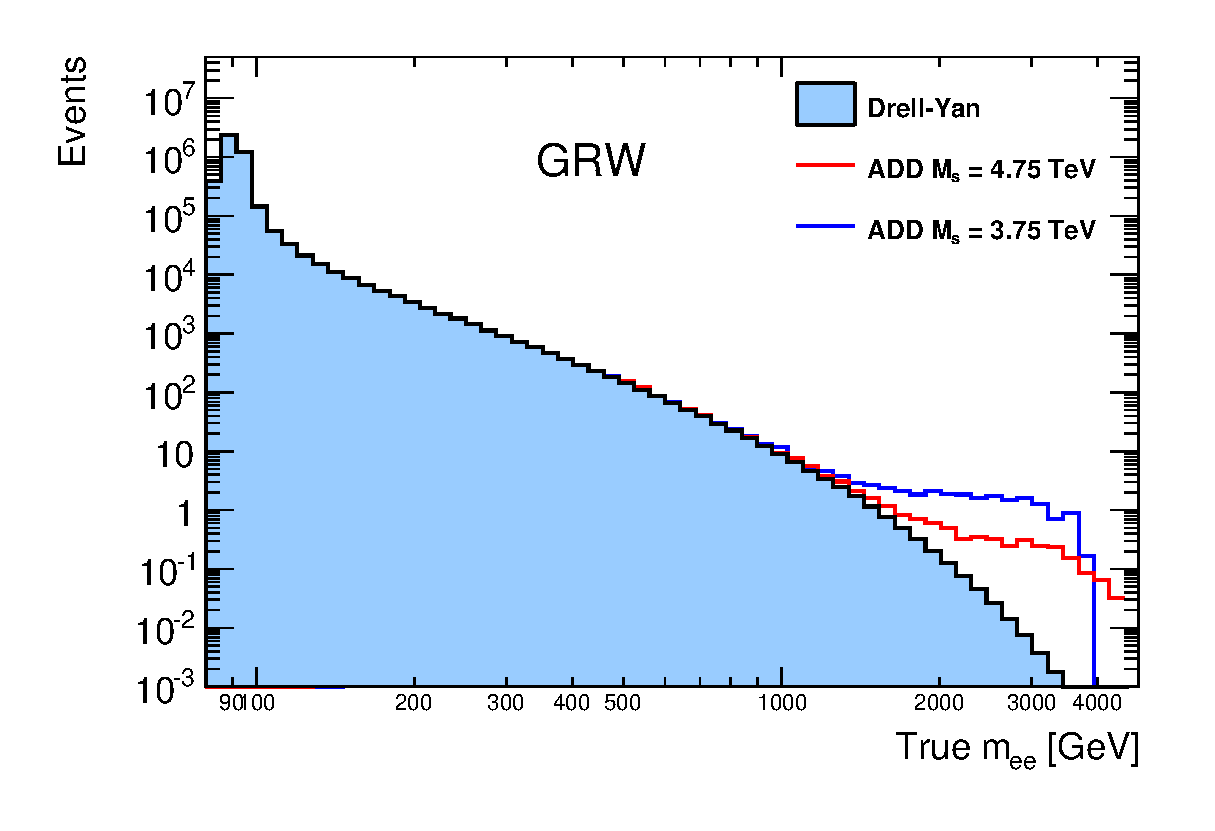
\includegraphics[width=0.9\linewidth]{images/truth_mass_ADD.eps}
            \end{center}
            \caption{MC truth level comparison between DY spectrum with and without ADD signal.}
            \label{fig:theoryInvMassADD}
        \end{figure}



\section{Past Searches}

    \subsubsection*{Contact Interaction}
        Several previous CI analyses have been done at hadron colliders including the LHC \cite{PhysRevD.87.015010,ATLAS:2012pu,PhysRevD.87.032001,PhysRevD.87.052017} and the Tevatron \cite{PhysRevLett.103.191803,PhysRevLett.96.211801,PhysRevLett.87.231803,PhysRevLett.82.4769,PhysRevLett.79.2198}. Searches were also performed at the electron-proton collider HERA \cite{Chekanov200423,Adloff200335}, previous lepton colliders \cite{Abdallah2009.60.1,Schael2007.49.411,Abdallah2006.45.589,Abbiendi2004.33.173,Acciarri200081} and neutrino scattering experiments \cite{}. Of the results comparable to this analysis searching for $qq\ell\ell$ contact interactions in the absence of signal the highest limits set on the scale of new physics $\Lambda$ come from the previous ATLAS analysis the author worked on \cite{PhysRevD.87.015010} detailed in chapter \ref{ch:7tev}. This analysis set a limit of $\Lambda$ $>$ 12.7~TeV and $\Lambda$ $>$ 9.63~TeV for the dilepton LL CI model for constructive and destructive interference respectively. The limits obtained for the electron channel for comparison to this analysis were $\Lambda$ $>$ 11.6~TeV for constructive and $\Lambda$ $>$ 8.76~TeV for destructive interference. By comparison the CMS results on the same 2011 data \cite{PhysRevD.87.032001} set limits of $\Lambda$ $>$ 13.1~TeV and $\Lambda$ $>$ 9.5~TeV for constructive and destructive isolation. Before the LHC the highest limits on $qq\ell\ell$ contract interactions came from the CDF at the Tevetron \cite{PhysRevLett.96.211801} that set limits on $qqee$ contact interactions for the LL, $\Lambda$ $>$ 5.9~TeV and $\Lambda$ $>$ 3.7 TeV, RR, $\Lambda$ $>$ 5.6~TeV and $\Lambda$ $>$ 3.9~TeV, and LR formalism, $\Lambda$ $>$ 5.8~TeV and $\Lambda$ $>$ 4.7~TeV, for constructive and destructive interference respectively. 


    \subsubsection*{ADD}
        The highest dilepton ADD limits set on the formalism normally used as a benchmark, GRW, are that of the previous ATLAS analysis on which the author worked \cite{PhysRevD.87.015010} discussed in chapter \ref{ch:7tev}. This analysis set a limit of M$_{S}$ $>$ 3.0~TeV on the scale of new physics (M$_{S}$). Other previous analyses have also been carried out searching for large extra dimensions with the ADD model. These analyses have come from the LHC \cite{}, from the Tevatron \cite{Abazov:2008as}, as well as from electron-proton collider HERA \cite{} and electron-positron collider LEP \cite{}. The highest limit before the LHC were those set by D0 on the Tevatron \cite{Abazov:2008as} which set limits of M$_{S}$ $>$ 1.45~TeV on the GRW model in the electron and photon channels. 








